% Journal of Economics (UGD) paper template. The journal takes Word files: see js-ugd-template.docx and README.md.
\documentclass[11pt,a4paper]{article}
\usepackage{js-ugd} % \usepackage[anonymous]{js-ugd} removes the authors for blind review
\addbibresource{references.bib}

\begin{document}

\JETitle{Title of the Paper in Title Case}
\JEAuthors{Firstname Lastname\textsuperscript{1}, Firstname Lastname\textsuperscript{2}}
\JEAffiliation{1}{Faculty, University, Street and number, City, Country}{first.author@example.com}
\JEAffiliation{2}{Faculty, University, Street and number, City, Country}{second.author@example.com}

\JEAbstract{Replace this text with the abstract. The abstract should be at least 250 and at most 500 words, including up to five keywords and keyphrases, and must fit on the first page of the paper.}

\JEKeywords{First keyword, Second keyword, Third keyword, Fourth keyword, Fifth keyword}

\section{Introduction}
\label{sec:intro}

Replace this text with your paper. Papers are submitted electronically through the journal's system, in Microsoft Word and PDF format. They should be from 8 to 12 pages long.

\section{Formatting Guidelines}
\label{sec:format}

Number sections 1, 2, 3 and subsections 1.1, 1.2, 1.3. Use a capital for the initial letter of every word in section and subsection titles.

\subsection{Text}

Write paragraphs in Arial 11, single-spaced, with no indent and fully justified. For emphasis on words or key terms, use italics, for example \emph{this is an emphasised text}. Do not use bold, underlining or another typeface.

\subsection{Tables}

Tables contain only horizontal rules. Each table needs a short descriptive title above it, column headings that clearly define the data, and all units of measurement. Put any footnotes below the table, and cite every table in the text. Number tables 1, 2, 3 and centre them with their captions. Place them in the text at the appropriate point, not at the end. For example, the margins of the page are set as in Table~\ref{tab:margins}.

\begin{table}[H]
\centering\jetablefont
\caption{Setup of margins for the paper}\label{tab:margins}
\begin{tabular}{p{4.2cm}p{4.2cm}}
\midrule
\textbf{Margin} & \textbf{Cm} \\ \midrule
Top & 2.5 \\ \midrule
Bottom & 2.5 \\ \midrule
Left & 2.5 \\ \midrule
Right & 2.5 \\ \midrule
Header & 1.25 \\ \midrule
Footer & 1 \\ \midrule
\end{tabular}
\end{table}

\subsection{Figures}

Centre figures and images, and place the caption after them. Number them 1, 2, 3, as in Figure~\ref{fig:example}.

\begin{figure}[H]
\centering
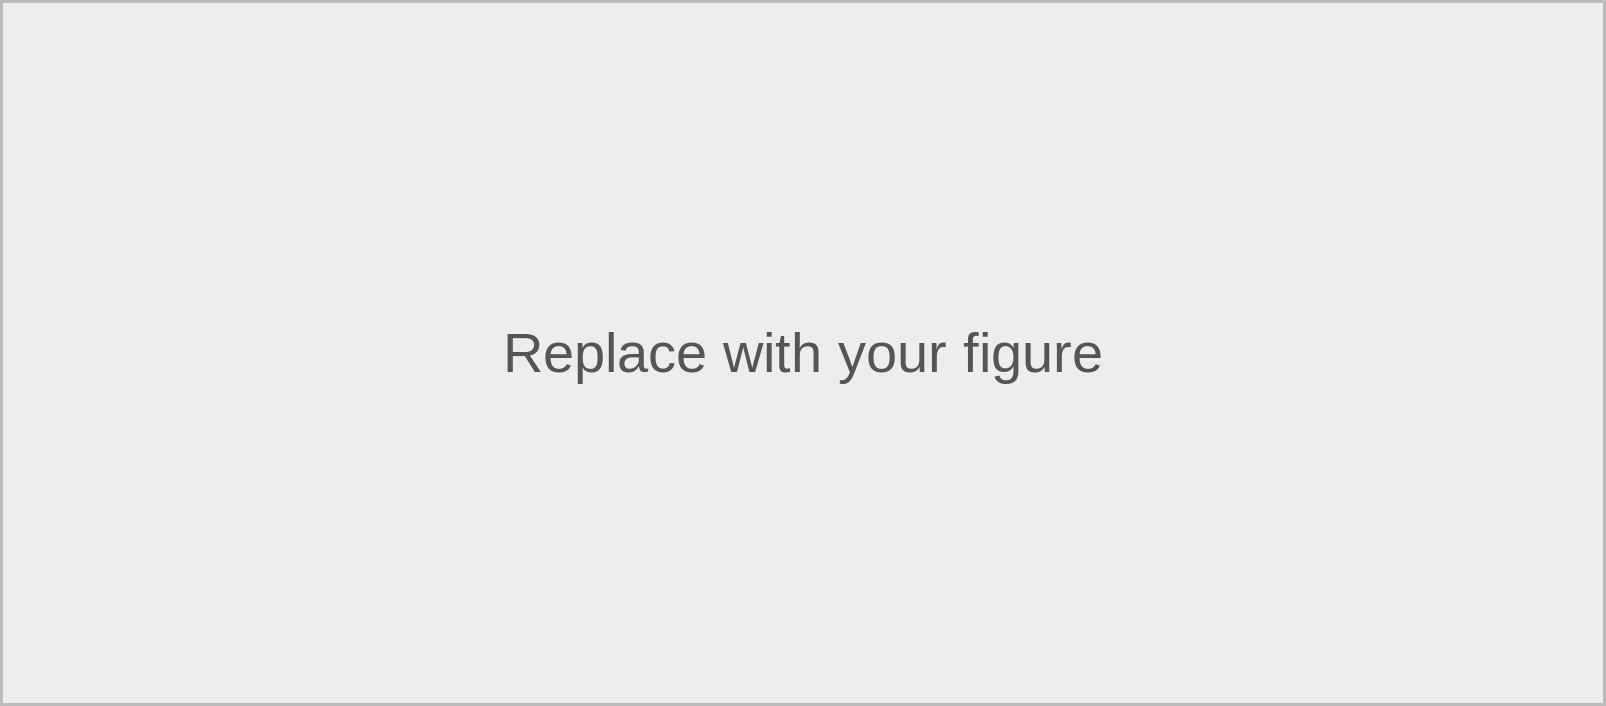
\includegraphics[width=13.6cm]{figure-placeholder.png}
\caption{Title of the figure}\label{fig:example}
\end{figure}

\subsection{Bullets}

A bullet list looks as follows:
\begin{itemize}
\item Bullet item one, some text;
\item Bullet item two, some other text.
\end{itemize}

\subsection{Equations}

Centre equations and number them at the right, as in equation~(\ref{eq:model}):
\begin{equation}
Y = \alpha + \beta X + \varepsilon
\label{eq:model}
\end{equation}

\subsection{Abbreviations}

As far as possible, avoid initials, except for terms in common use. Spell abbreviations out the first time they are mentioned, with the abbreviation in brackets, as in Goce Delcev University (UGD). List them in alphabetical order before the references.

\subsection{Citations and References}

Use APA style in the text. A parenthetical citation has the surname and the year: \parencite{taylor1993} for one author, \parencite{dieboldli2006} for two, and \parencite{clarida2000} for three or more. A narrative citation has the surname and the year in brackets: \textcite{taylor1993}.

In the reference list, references are numbered, listed in APA style and alphabetized by the last name of the first author. Every reference in the text must be in the list, with its URL where available. The list below has a journal article \parencite{veselinova2025}, a book \parencite{hamilton1994}, a working paper \parencite{svensson1994} and a webpage \parencite{jesubmissions}.

\section{Conclusions}
\label{sec:concl}

Replace this text with your conclusions.

\section*{Abbreviations}

APA: American Psychological Association; UGD: Goce Delcev University.

\section*{References}
\printbibliography[heading=none]

\end{document}
